\documentclass[11pt]{article}
\usepackage{amsmath,amssymb,amsthm,amsfonts,hyperref,graphicx,verbatim,float,microtype,cite, lmodern,titlesec,multicol,subfig}
%\usepackage[dvipsnames]{xcolor}
\usepackage[left=1.5cm,right=1.5cm,top=1.5cm,bottom=1.5cm]{geometry}
\usepackage[none]{hyphenat}
\usepackage[justification=centering]{caption}
\pagenumbering{gobble}
\thispagestyle{empty}
\renewcommand{\baselinestretch}{1.2}
\setlength{\parindent}{0pt}
\setlength{\columnsep}{20pt}

\titleformat{\section}[display]
  {\normalfont\fillast}
  {\large\scshape section \oldstylenums{\thesection}}
  {1ex minus .1ex}
  {\large\scshape}
\titlespacing{\section}{3pc}{*1}{*1}[3pc]
\titlespacing{\paragraph}{0pc}{*.5}{*.5}[3pc]


%%% Math:
\newcommand{\p}{\mathbb{P}}
\newcommand{\indep}{\mathrel{\perp\mspace{-10mu}\perp}}
\newcommand{\nindep}{\centernot{\indep}}


%%%%%%%%%%%%%%%%%%%%%%%%%%%%%%%%%%%%%%%%%%%%%%%%%%%%%%%%%%%%%%%%%%%%%%%%%%%%%%%%%%%%%%%%%%%
%						                   Header										  %
%%%%%%%%%%%%%%%%%%%%%%%%%%%%%%%%%%%%%%%%%%%%%%%%%%%%%%%%%%%%%%%%%%%%%%%%%%%%%%%%%%%%%%%%%%%

\begin{document}
{\scshape{\LARGE[MVA] Probabilistic Graphical Models}\rule{4.4cm}{.4pt}[12/12/15]}\\
\begin{minipage}[t]{6cm}
\flushleft
Project progress
\end{minipage}
\null\hfill
\begin{minipage}[r]{6cm}
\flushright
  Maha ELBAYAD
\end{minipage}
\begin{center}
\scshape{\LARGE A tree based context model \\for Object Recognition}\\
\end{center}
\vspace{10pt}
%%%%%%%%%%%%%%%%%%%%%%%%%%%%%%%%%%%%%%%%%%%%%%%%%%%%%%%%%%%%%%%%%%%%%%%%%%%%%%%%%%%%%%%%%%%
%						                   Core  										  %
%%%%%%%%%%%%%%%%%%%%%%%%%%%%%%%%%%%%%%%%%%%%%%%%%%%%%%%%%%%%%%%%%%%%%%%%%%%%%%%%%%%%%%%%%%%
\begin{multicols}{2}
\section*{Introduction}
The probabilistic framework presented in \cite{htree} aims to exploit contextual information in addition to local features to detect and localize multiple object categories coexisting in an image.
\section*{The model}
The model consists of two major components:
\paragraph*{Prior model} whose role is to capture dependencies between object categories. Learning this model breaks down to the following steps:

$\bullet$ Learning the dependency structure from co-occurrences of object pairs in a set of fully labeled images via Chow-liu's algorithm\cite{chowliu}.
A node $b_i$ in the tree is a binary variable indicating the presence of the object $i$ in the image.
From the tree structure, the joint probability of $b=(b_i)_i$ is given by:
\[\p(b)=\p(b_{root})\prod_i\p(b_i|b_{\pi_i})\]
$\bullet$ Learning the location prior: each object's location in an image is encoded with 3 coordinates\cite{3D}:
\[(L_x,L_y,L_z)=(l_x,l_y,1).\frac{H_i}{l_h}\tag{fig \ref{3D}}\]
The final adopted location variable for object category i would be\footnote{$L_x$ dropped given that horizontal locations have weak contextual information}:
\[L_i=(L_y,\log L_z)\]
Assuming $(L_y^{(i)})_i$, $(\log L_z^{(i)})_i$ are jointly Gaussians and that when $L=(L_i)_i$ is conditionned on the r.v $b$, it inherits the same dependency tree structure (figure \ref{tree}). 

Thus:
\[\p(L|b)=\p(L_{root}|b_{root})\prod_i\p(L_i|L_{\pi_i},b_i,b_{\pi_i})\] 
\paragraph*{Measurement model} which encompasses the global gist descriptor \cite{gist} of the image plus the outputs of local detectors for each object category $(i)$, that is a list of $K_i$ candidates $(W_{ik},s_{ik})_{k=1:K_i}$, $W_{ik}=(L_y,\log L_z)$ parametrizes the bounding box and $s_{ik}$ is a detection score. Those predictions are then assessed on the training set yielding the binary variable $\forall i,k\:c_{ik}=$\texttt{is\_correct\_detection}.
\section*{Learning}
We first estimate $\p(L_i|L_{\pi_i},b_i,b_{\pi_i})$ as three gaussians: (1) the case $(b_i=1,b_{\pi_i}=1)$ as $L_i|L_{\pi_i}$. (2) the case $(b_i=1,b_{\pi_i}=0)$ as $L_i\indep L_{\pi_i}$ and (3) the case $(b_i=0)$ as $L_i\indep L_j\:\forall j$ and set $L_i=\mathbb E_{images}(L_i)$

For the gist decriptor, we use logistic regression to fit $\p(b_i|g)$ and we handle the local detectors similarly to fit $\p(c_{ik}|s_{ik})$.

\textbf{Alternating inference on trees:} Now that we lerned our parameters $g,s$ and $W$ we solve for $b,c$ and $L$ as:
\[\hat b,\hat c,\hat L=\arg\max_{b,c,L}\p(b,c,L|g,s,W)\]
We infer the optimal values iteratively:

(a\footnote{For the first iteration we set $\hat b,\hat c=\arg\max_{b,c}\p(b,c|g,s)$}): $\hat b,\hat c=\arg\max_{b,c}\p(b,c|g,s,W,\hat L)$

\section*{Preliminary results}
Currently at the training phase on the $SUN-09$ database (111 categories, 4317 images). A subtree of the inferred dependency tree is shown in figure \ref{sky}.
\end{multicols}
%%%%%%%%%%%%%%%%%%%%%%%%%%%%%%%%%%%%%%%%%%%%%
%    				Figures
%%%%%%%%%%%%%%%%%%%%%%%%%%%%%%%%%%%%%%%%%%%%%

\begin{figure}[H]
\centering
\subfloat[3D world coordinates\label{3D}]{
	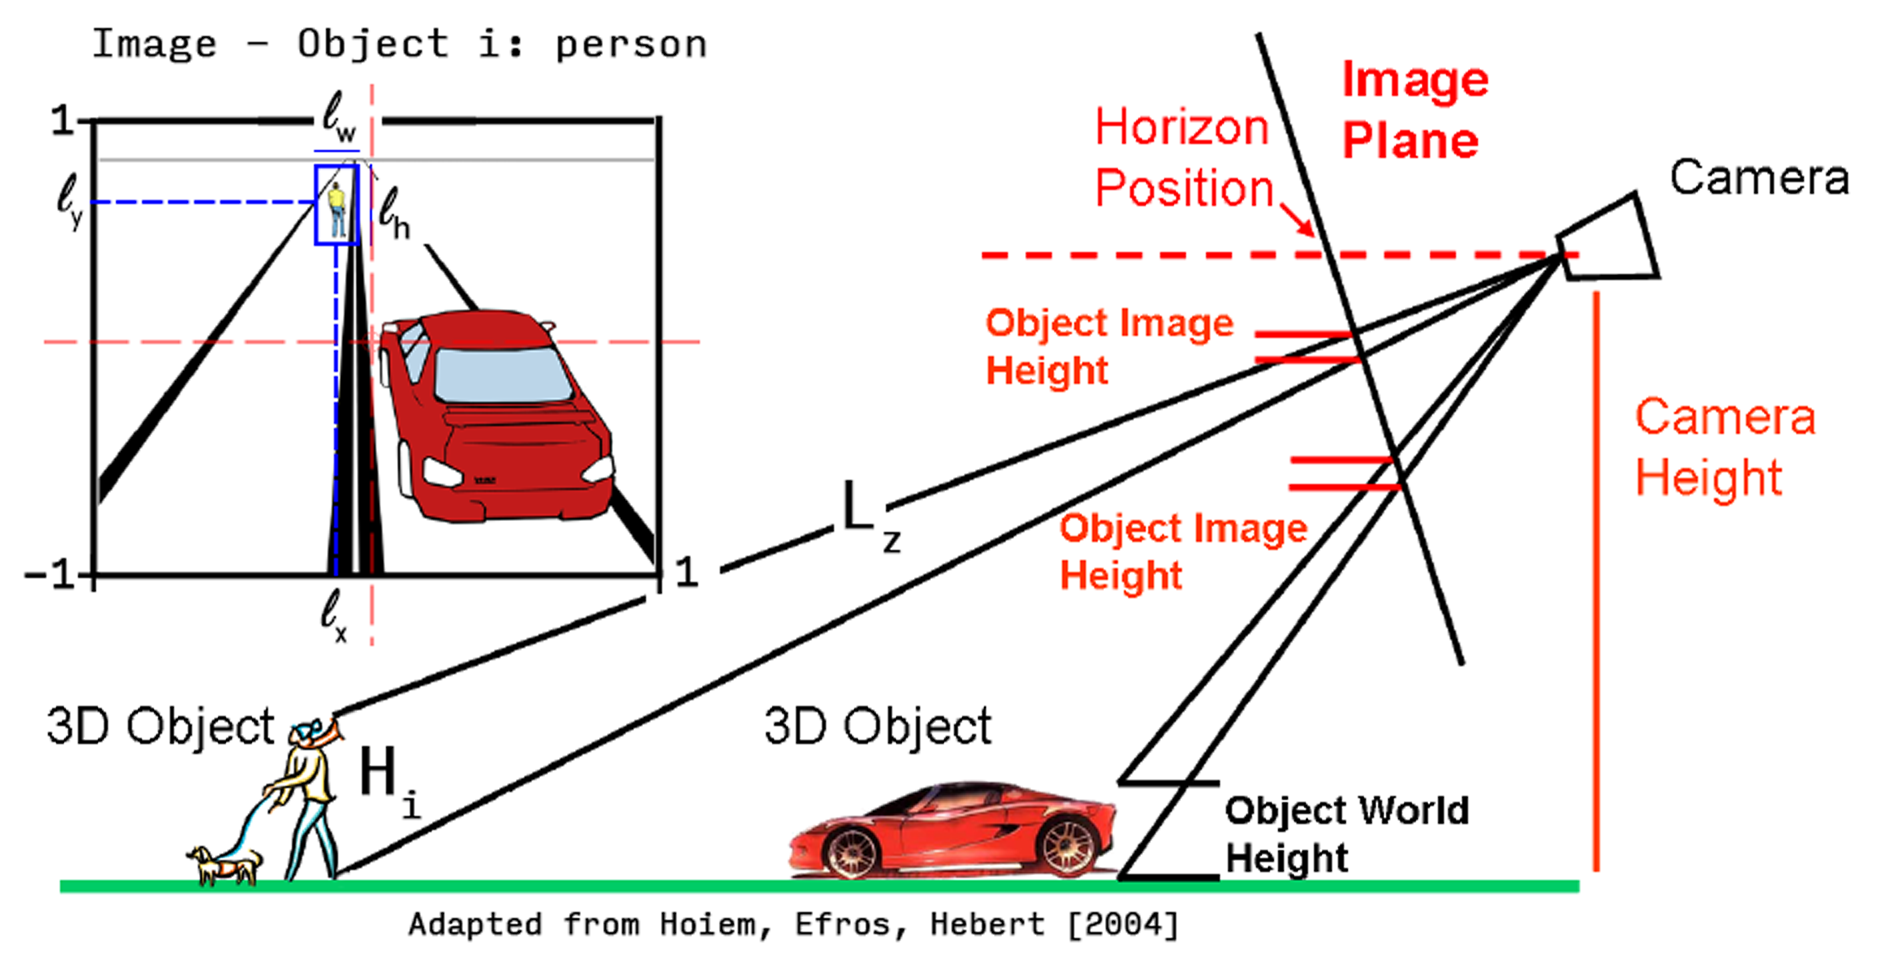
\includegraphics[width=10cm]{images/3DC.png}
}
\subfloat[Prior model - Tree structure\label{tree}]{
	\includegraphics[width=10cm]{images/tikz1.pdf}
}
\caption{}
\end{figure}

\begin{figure}[H]
\centering
\includegraphics[width=16cm]{images/sky_tree.png}
\caption{\small (Sky) subtree considering (Floor) as the root of the tree\label{sky}\\
Red edges:(-) correlation -  Blue edges: (+) correlation\\ The line width reflects the probability of co-occuring }
\end{figure}
%%%%%%%%%%%%%%%%%%%%%%%%%%%%%%%%%%%%%%%%%%%%%
%    				Biblio
%%%%%%%%%%%%%%%%%%%%%%%%%%%%%%%%%%%%%%%%%%%%%

\begin{thebibliography}{2}
\bibitem{htree} Choi, M. J., Torralba, A., \& Willsky, A. S. (2012). A tree-based context model for object recognition. Pattern Analysis and Machine Intelligence, IEEE Transactions on, 34(2), 240-252.

\bibitem{chowliu}Chow, C. K., \& Liu, C. N. (1968). Approximating discrete probability distributions with dependence trees. Information Theory, IEEE Transactions on, 14(3), 462-467.

\bibitem{3D}Hoiem, D., Efros, A. A., \& Hebert, M. (2008). Putting objects in perspective. International Journal of Computer Vision, 80(1), 3-15.

\bibitem{gist}Torralba, A. (2003). Contextual priming for object detection. International journal of computer vision, 53(2), 169-191.
\end{thebibliography}

\end{document}

